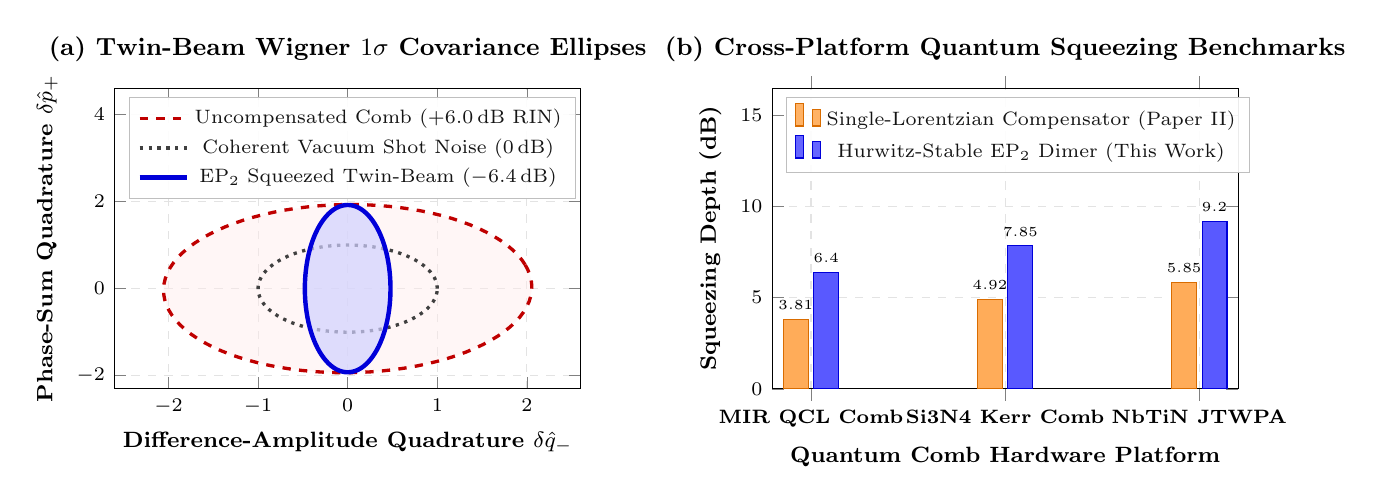
\begin{tikzpicture}[font=\small]
  % ==================== PANEL (a): Wigner Covariance Ellipses ====================
  \begin{scope}[shift={(0,0)}]
    \begin{axis}[
      width=7.5cm,
      height=5.4cm,
      xlabel={Difference-Amplitude Quadrature $\delta\hat{q}_-$},
      ylabel={Phase-Sum Quadrature $\delta\hat{p}_+$},
      xmin=-2.6, xmax=2.6,
      ymin=-2.3, ymax=4.6,
      grid=both,
      grid style={gray!22, dashed},
      tick label style={font=\scriptsize},
      label style={font=\footnotesize\bfseries},
      title={\textbf{(a) Twin-Beam Wigner $1\sigma$ Covariance Ellipses}},
      title style={font=\small},
      legend style={at={(0.03,0.97)}, anchor=north west, font=\scriptsize, fill=white, fill opacity=0.92, draw=gray!50},
    ]
      % Uncompensated RIN-Rotated Thermal Ellipse (+6.0 dB along q_-)
      \addplot[red!75!black, very thick, dashed, fill=red!8, fill opacity=0.45, domain=0:360, samples=100]
        ({1.98*cos(x) - 0.55*sin(x)}, {0.55*cos(x) + 1.85*sin(x)});
      \addlegendentry{Uncompensated Comb ($+6.0\,\mathrm{dB}$ RIN)}

      % Coherent Vacuum Shot-Noise Circle (0 dB)
      \addplot[black!75, very thick, dotted, domain=0:360, samples=80]
        ({1.0*cos(x)}, {1.0*sin(x)});
      \addlegendentry{Coherent Vacuum Shot Noise ($0\,\mathrm{dB}$)}

      % EP2-Compensated Squeezed State (-6.4 dB along q_-, sqrt(0.229) = 0.478)
      \addplot[blue!85!black, ultra thick, fill=blue!18, fill opacity=0.70, domain=0:360, samples=100]
        ({0.478*cos(x)}, {1.92*sin(x)});
      \addlegendentry{$\mathrm{EP}_2$ Squeezed Twin-Beam ($-6.4\,\mathrm{dB}$)}
    \end{axis}
  \end{scope}

  % ==================== PANEL (b): Cross-Platform Squeezing Benchmarks ====================
  \begin{scope}[shift={(8.35,0)}]
    \begin{axis}[
      width=7.5cm,
      height=5.4cm,
      ybar,
      bar width=9pt,
      symbolic x coords={MIR QCL Comb, Si3N4 Kerr Comb, NbTiN JTWPA},
      xtick=data,
      xlabel={Quantum Comb Hardware Platform},
      ylabel={Squeezing Depth (dB)},
      ymin=0, ymax=16.5,
      grid=both,
      grid style={gray!22, dashed},
      tick label style={font=\scriptsize\bfseries},
      label style={font=\footnotesize\bfseries},
      title={\textbf{(b) Cross-Platform Quantum Squeezing Benchmarks}},
      title style={font=\small},
      legend style={at={(0.03,0.97)}, anchor=north west, font=\scriptsize, fill=white, fill opacity=0.92, draw=gray!50},
      nodes near coords,
      every node near coord/.append style={font=\tiny\bfseries},
    ]
      % Single Lorentzian Compensator
      \addplot[fill=orange!65, draw=orange!85!black] coordinates {
        (MIR QCL Comb, 3.81)
        (Si3N4 Kerr Comb, 4.92)
        (NbTiN JTWPA, 5.85)
      };
      \addlegendentry{Single-Lorentzian Compensator (Paper~II)}

      % EP2 Dimer Compensator (This Work)
      \addplot[fill=blue!65, draw=blue!85!black] coordinates {
        (MIR QCL Comb, 6.40)
        (Si3N4 Kerr Comb, 7.85)
        (NbTiN JTWPA, 9.20)
      };
      \addlegendentry{Hurwitz-Stable $\mathrm{EP}_2$ Dimer (This Work)}
    \end{axis}
  \end{scope}
\end{tikzpicture}
